\documentclass[../../main.tex]{subfiles}
\usetikzlibrary{patterns}
\begin{document}

{\bf [解]}
題意の条件文は以下の3つである．
\begin{align}
& x > 0, y > 0, a > 0 \label{eq:1} \\
& x + y \le 1 + a \label{eq:2} \\
& \dfrac{1}{x} + \dfrac{1}{y} \le 4(1+a) \label{eq:3}
\end{align}
ここから$y$を消去していくことによって題意を示す．
まず\cref{eq:2}を$y$について整理して
\begin{align}
 y \le 1 + a - x \label{eq:4}
\end{align}
である．
次に\cref{eq:3}を$y$について整理すると\cref{eq:1}に注意して
\begin{align}
 \dfrac{1}{y} \le 4(1+a) - \dfrac{1}{x} \\
\therefore 
 0 < \dfrac{1}{4(1+a) - \dfrac{1}{x}} \le y  \label{eq:5}
\end{align}
である．
\cref{eq:4,eq:5}を\cref{eq:1}に代入して $y$ の存在条件を考えると，$y$が存在するための条件は
\begin{align}
& 0 < 1 + a - x \label{eq:6} \\
& 0 < \dfrac{1}{4(1+a) - \dfrac{1}{x}} \\
& \dfrac{1}{4(1+a) - \dfrac{1}{x}} \le 1 + a - x \label{eq:7} 
\end{align}
である．
\cref{eq:7}を整理すると
\begin{align}
 1 \le (1+a-x) \left\{ 4(1+a) - \dfrac{1}{x} \right\} = -4(1+a)x - \dfrac{1+a}{x} + 1 + 4(1+a)^2
\end{align}
だから両辺に $x (>0)$ をかけて
\begin{align}
0 \le -4(1+a)x^2 + 4(1+a)^2 x - (1+a) 
\end{align}
を得る．\cref{eq:1}より$1+a > 0$ だから両辺 $(1+a)$ でわって
\begin{align}
&4x^2 - 4(1+a)x + 1 \le 0 \\
&(2x - 1)^2 \le 4ax 
\end{align}
となる．右辺に\cref{eq:6}を用いて
\begin{align}
 (2x - 1)^2 < 4a(1+a) 
\end{align}
だから題意は示された．

{\bf [解説]}
解答では数式変換だけに頼って解いたが，図示した方がミスは起こりにくいだろう．
与えられた領域\cref{eq:1,eq:2,eq:3}を$xy$平面に図示すると下図の斜線部のようになる．
緑の線が
\begin{align}
 y = (2x-1)^2 -4a(a+1)
\end{align}
を表しており，斜線部の$x$の範囲では常に$y<0$をとっていることがわかるから，よってグラフより題意は示される．
（もちろん解答にするときはちゃんと負になることを示さないといけない．）
結局問題なのは二つの曲線
\begin{align}
 x+y = 1+a \\
 \dfrac{1}{x} + \dfrac{1}{y} = 4(1+a)
\end{align}
の交点を求めるのが計算上面倒臭いという点で，そこさえクリアできれば解法自体は単純だ．


\begin{figure}[htb]
 \begin{center}
  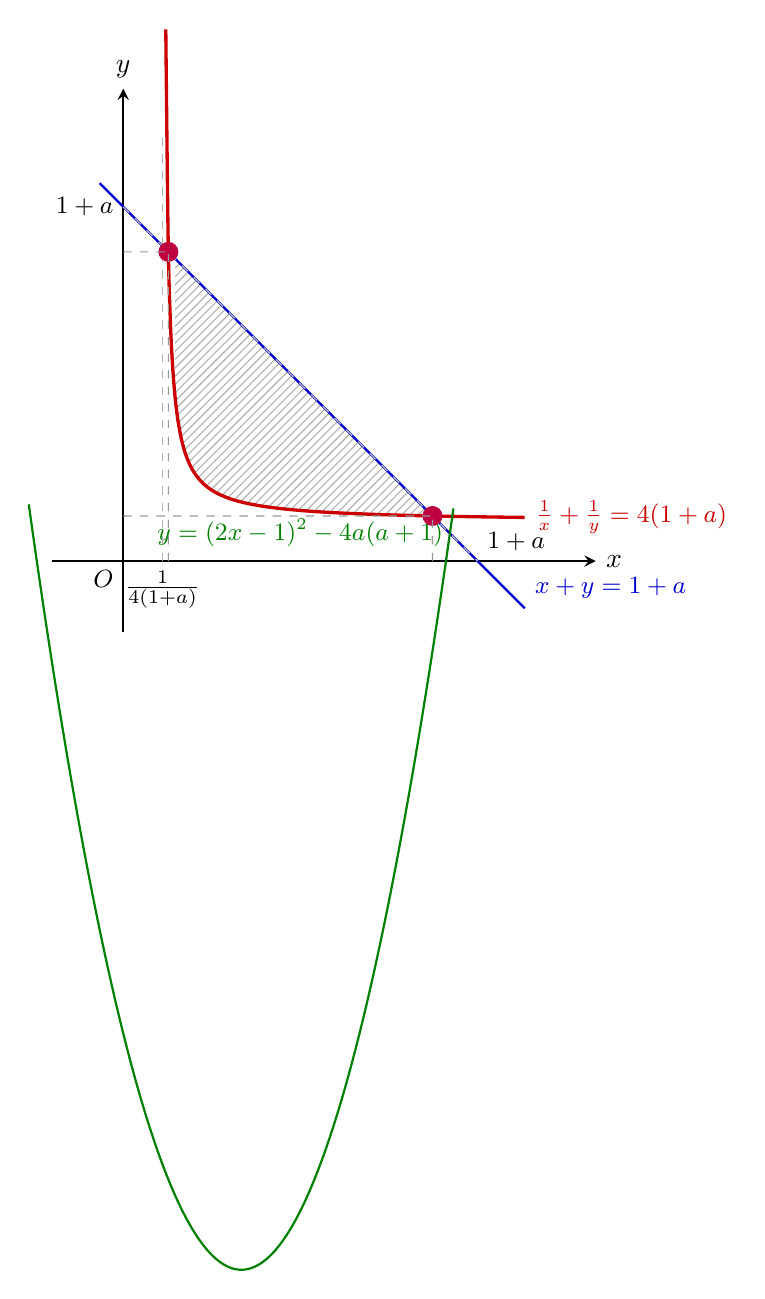
\begin{tikzpicture}[scale=3, >=stealth]
    % パラメータ a の設定 (例として a = 0.5 と設定: 1+a = 1.5)
    \def\A{1.5} % 1 + a

    % 軸の描画
    \draw[->, thick] (-0.3, 0) -- (2.0, 0) node[right] {$x$};
    \draw[->, thick] (0, -0.3) -- (0, 2.0) node[above] {$y$};
    \node[below left, font=\small] at (0,0) {$O$};

    % -------------------------------------------------------------
    % 領域のハッチング（斜線塗りつぶし）
    % 境界: (x1, y1) から x に沿って直線と曲線の交点・端点まで
    % -------------------------------------------------------------
    % 領域: x in [0.22, 1.28] 付近で 
    % 上側: y = (1+a) - x
    % 下側: y = x / (4*(1+a)*x - 1)
    
    % pattern = north east lines (右上上がりの斜線)
    \fill[pattern=north east lines, pattern color=gray!60]
        plot[domain=0.22:1.28, samples=100]
            (\x, {\x / (4*\A*\x - 1)}) % 下側の曲線
        -- plot[domain=1.28:0.22, samples=2]
            (\x, {\A - \x})            % 上側の直線
        -- cycle;

    % -------------------------------------------------------------
    % 境界線の描画
    % -------------------------------------------------------------

    % 1. 直線 x + y = 1 + a
    \draw[thick, blue!80!black, domain=-0.1:1.7] 
        plot (\x, {\A - \x}) node[above right, font=\small] {$x + y = 1 + a$};

    % 2. 曲線 1/x + 1/y = 4(1+a)  <=>  y = x / (4(1+a)x - 1)
    % x > 1/(4(1+a)) = 1/6 ≒ 0.167 の範囲で描画
    \draw[very thick, red!80!black, domain=0.18:1.7, samples=150, smooth] 
        plot (\x, {\x / (4*\A*\x - 1)}) 
        node[right, font=\small] {$\frac{1}{x} + \frac{1}{y} = 4(1+a)$};

    % 3. 放物線 y = (2x-1)^2 - 4a(a+1)
    % a=0.5 のとき y = (2x-1)^2 - 3
    \draw[thick, green!50!black, domain=-0.4:1.4, samples=200, smooth]
        plot (\x, {(2*\x - 1)^2 - 4*(\A-1)*\A})
        node[below left, font=\small] {$y = (2x-1)^2 - 4a(a+1)$};

    % 漸近線 x = 1 / 4(1+a)
    \draw[dashed, gray!60] ({1/(4*\A)}, 0) node[below, black] {$\frac{1}{4(1+a)}$} 
        -- ({1/(4*\A)}, 1.8);


    % 軸上の切片と破線
    \draw[dashed, gray!60] (0, \A) node[left, font=\small, black] {$1+a$} -- (\A, 0) node[above right, font=\small, black] {$1+a$};

    % % 領域ラベル
    % \node[font=\small, purple!80!black, fill=white] at (0.75, 0.55) {領域 $D$};

    % 交点1 (x が小さい方の交点: x ≒ 0.191, y ≒ 1.309)
    \coordinate (P1) at (0.191, 1.309);
    \fill[purple] (P1) circle (1.2pt);
    \draw[dashed, gray!80] (0.191, 0) -- (P1);
    \draw[dashed, gray!80] (0, 1.309) -- (P1);
    
    % 交点2 (x が大きい方の交点)
    % a=0.5 (1+a=1.5) のとき 4x^2 - 6x + 1 = 0 より x = (3+sqrt(5))/4 ≒ 1.309
    \coordinate (Q) at (1.309, {\A - 1.309});
    \fill[purple] (Q) circle (1.2pt);
    \draw[dashed, gray!80] (1.309, 0) -- (Q);
    \draw[dashed, gray!80] (0, {\A - 1.309}) -- (Q);



\end{tikzpicture}
\caption{$x,y$の存在領域}
\end{center}
\end{figure}

\newpage

\end{document}
